\section{Evaluation}
\label{eval}

In this section, we describe our empirical evaluation on the detection
accuracy of {\model} in comparison with the state-of-the-art,
SVM-based approach by Sun {\em et al.}~\cite{davidlo10}. All of
experiments were carried out on on a computer with CPU AMD Phenom II
X4 965 3.0 GHz, 8GB RAM, and Windows~10.

%We also re-implemented the machine learning approach described in
%their paper~\cite{davidlo10} using SVM in LIBSVM tool.

\subsection{Data Sets and Feature Extraction}

%\begin{table}[t]
%\centering
%\caption{Statistics of All Bug Report Data}
%    \begin{tabular}{lcrrr}
%    \hline
%    Project &  Time period &  Report &  Duplicate &  Term \\
%    \hline
%    Eclipse  &  06/29/2008 - 06/28/2010 & 6,100 & 981 & 22,558 \\
%    OpenOffice & 04/12/2010 - 04/10/2011 & 7,000 & 338 & 22,051 \\
%    Firefox  &  01/26/2011 - 04/11/2011 & 20,000 & 936 & 42,515 \\
%    Apache  &  11/19/2006 - 03/30/2011 & 10,000 & 494   & 34,850 \\
%    FreeDesktop &  01/25/2010 - 04/13/2011 & 10,000 & 543   & 33,068 \\
%    NetBeans    & 06/17/2010 - 04/13/2011 & 10,000 & 993 & 27,417\\
%    \hline
%    \end{tabular}%
%\label{data}
%\end{table}

\begin{table}[t]
\addtolength{\tabcolsep}{-3pt}
\centering
\small
\caption{Statistics of All Bug Report Data}
    \begin{tabular}{lcccccc}
    \hline
    Project &  Time period &  Report &  Dup  & Train & Test \\
    \hline
    OpenOffice & 01/01/2008 - 12/21/2010 & 31,138 & 3,371 & 200 & 3,171  \\
    Moz. FireFox &  01/01/2010 - 12/31/2010 & 75,653 & 6,925 & 200 & 6,725 \\
    Eclipse  &  01/01/2008 - 12/31/2008 & 45,234 & 3,080 & 200 & 2,880  \\
    \hline
    Apache  &  11/19/2006 - 03/30/2011 & 10,000 & 494   & 200 & 3,485 \\
    FreeDesktop &  01/25/2010 - 04/13/2011 & 10,000 & 543   & 200 & 3,306 \\
    NetBeans    & 06/17/2010 - 04/13/2011 & 10,000 & 993 & 200 & 2,741\\
    \hline
    \end{tabular}
\label{data}
\end{table}

For the comparison purpose, we chose the same data sets of bug reports
used in the existing work~\cite{davidlo10} (Table~\ref{data}).
%We used the same data sets of bug reports in the open-source projects
%as in REP~\cite{sun-ase11} (Table~\ref{data}). 
Column \code{Time period} displays the time period of collected bug
reports. Columns \code{Report} and \code{Dup} show the numbers of bug
reports and duplicate ones, respectively. Columns \code{Train} and
\code{Test} show the number of the duplicate bug reports used for
training and testing, respectively. Each bug report has its unique
ID, a summary, a description, comments, and other metadata
(e.g., severity, priority, its reporter, creation date, etc). All
projects are developed in a long history.  
%
%The duplication information among bug reports is also available in
%that data set.
The information on the duplications is available in the 
collected bug reports. 
Each duplicate report is marked and links to its duplicate group. The
data is used to train {\model} and ensemble weights, and then used to
evaluate {\model}'s accuracy in detecting the duplication between a
bug report and the duplicate bug report~groups.
%-------------------------------------------------

%We conducted an empirical evaluation of {\model} on several
%open-source systems. We collected the data from the bug repositories
%of the systems (Table~\ref{data}). Column \code{Time period} displays
%the time period of collected bug reports. Columns \code{Report} and
%\code{Duplicate} show the numbers of bug reports and duplicate ones,
%respectively.
%For Eclipse, we chose Eclipse' s platform component from October 2000
%to July 2010 with 61,110 bug reports, in which 14,020 are determined
%by Eclipse's developers as duplicate ones. For Jazz project from June
%2005 to June 2008, the total number of bug reports are 34,228, in
%which 874 of them are recorded as duplications. 
%Each bug report has its unique ID, a summary, a description, comments,
%and other metadata (e.g. severity, priority, its reporter, creation
%date, platform, etc).


The summary and description of a bug report were merged and considered
as a document. It then went through pre-processing such as stemming,
and removing grammatical and stopwords, and single-occurrence words
as in~\cite{davidlo10}.
In our experiment, for {\model}, we extracted and merged the summary
and description of each report, and used the merged contents as the
document for the report. Each document was then preprocessed such as
stemming for term normalization, and removing grammatical words
(e.g., ``a'', ``the'', ``and'', etc.) and those terms appearing once in
the entire corpus as in~\cite{RTM}. Tf-Idf was run to determine and
remove the common words that appear in most of the bug reports.
Then, all the words were collected and indexed into a vocabulary.
After this phase, a bug report is represented as a vector of the
indexes of its words in the vocabulary. After this phase, a bug report is
represented as a vector of indexes of its words in the vocabulary and
is used in the model. Duplication information among bug reports was
also extracted from the repositories.

%In our experiment, we extracted and merged the summary and description
%of each report, and used the merged contents as the document for the
%report. Each document was then preprocessed such as stemming for term
%normalization, and removing grammatical words (e.g. ``a'', ``the'',
%``and'', etc) and those terms appearing once in the entire corpus as
%in~\cite{RTM}.
%%%This phase include stemming for term normalization, removing
%%%grammatical words (e.g. ``a'', ``the'', ``and'', etc) and those that
%%%appear once in the entire corpus or appear in almost all
%%%documents.
%Then, all the words were collected and indexed into a vocabulary.
%Column \code{Term} shows the number of extracted terms in each
%vocabulary set after pre-processing. After this phase, a bug report is
%represented as a vector of indexes of its words in the vocabulary and
%is used in the model. Duplication information among bug reports was
%also extracted from the repositories.


%%%That is, a document of bug report $d$ with $N$ words will have the
%%%form ${\bf{w}}_d=(w_{d0}, w_{d1}, ..., w_{dN})$ where $w_{dk}$ is the
%%%index of the word at position $k$ in the vocabulary.
%%%The link indicator for $d$ with another bug report $d'$ will take the
%%%value of 1 if they are duplicate, otherwise, it will take the value of
%%%0. The vectors of bug reports and the values for the link indicators
%%%were used as features in training {\model}.

%This vector and the link indicator of the duplicate reports of $d$
%with all other known bug reports $d'$, which take value of $1$ if $d$
%is a duplicate of $d'$ and $0$ otherwise, will be applied to the input
%of iRTM.

\subsection{Evaluation Setup and Metrics}

For the purpose of comparing the performance of {\model} with that of
other work, we use the same evaluation metrics and setup as in the
previous research of Sun {\em et al.}~\cite{davidlo10} for duplicate
bug report detection. 
%
%Tien
%The evaluation setting is the same as in REP~\cite{sun-ase11}.  
Specifically, all bug reports were sorted in the chronological
order. We divided the data set into two sets.  The training set
includes the first $M$ reports in the repository, of which 200 reports
are duplicates.  It was used to train the parameters for the
models. The remaining reports were used for testing. At each
execution, we ran {\model} through the testing reports in the
chronological order. When it determines a duplicate report $b$, it
returns the list of top-$k$ potential duplicate report groups. If a
true duplicate report group $G$ is found in the top-$k$ list, we count
it as a hit. We then added $b$ to that group for later training. The
top-$k$ accuracy (i.e. recall rate) is measured by the ratio of the
number of hits over the total number of considered bug reports.  After
each frame, we incrementally updated {\model} and re-trained the SVM
model in Sun {\em et al.}'s.


%Due to un-availability of their tool, we re-implemented the SVM-based
%machine learning approach described in their paper~\cite{davidlo10}
%using LIBSVM tool~\cite{libsvm}. The authors of that work used LIBSVM
%to implement their approach. They also used that setup to compare
%their approach with other state-of-the-art approaches. The same
%longitudinal setup was used in our experiment, simulating the usage of
%our {\model} tool in reality. That is, bug reports were sorted
%according to the chronological order, and then divided into 10
%non-overlapped and equally sized frames. Each frame was indexed
%corresponding to their creation time.

%Thus, bug reports in frame $i-1$ were created before bug reports in
%frame $i$.

%Initially, frame $0$ with its bug reports and their duplication
%indicators were used for training {\model} (Phase 1). Then, we used
%the model to test each bug report $d$ in frame $1$ (Phase 2). Our
%model gave a top list of $T$ bug reports that were filed before $d$
%(in both frames $0$ and $1$) and were likely to be the duplications of
%$d$. If the list contains at least one bug report that is a true
%duplication of $d$, we count this as {\em a hit} (i.e. a correct
%detection). After that, we updated the model (Phase 3) with new data
%in frame $1$, including all bug reports in frame $1$ and all true
%duplication indicators within both frames $0$ and $1$. The updated
%model was then used to test frame $2$. We continued in the same way
%for the remaining frames. For Sun {\em et al.}'s, after each frame, we
%completely re-trained the SVM model.
%After each frame, we incrementally updated
%{\model} and re-trained the SVM model in Sun {\em et al.}'s.
%At last, we calculated \emph{accuracy}, i.e. the ratio of the number
%of hits over the total number of true duplicate bug reports under
%test, as in Sun {\em et al.}~\cite{davidlo10}. The {\em top-ranked}
%({\em top-T}) accuracy was calculated for each value of cut point $T$
%from 1 to 10.



We chose the top-ranked accuracy as a performance metric, rather than
precision (i.e., the ratio between the number of correctly detected ones
over the total number of detected ones) and recall (i.e., the ratio
between the number of correctly detected ones over the total number of
duplicate ones). The reason is that using detection accuracy fits
better in evaluating this detection tool: given a new bug report, a
tool returns a list of ranked bug report candidates that could
potentially be a duplication of the given report.
%That is, the goal aimed to evaluate how likely the real duplicate bug
%report of the given bug report is in the top-$T$ results. 
Recall does not reflect well the quality of this type of tool because
the tool can return a very long list of results with the top-ranked
results containing the correct duplicate one of the given bug
report. In such cases, recall is very low, however, the tool is very
useful.


%In this case, data in frame $1$ is updated into the model trained from frame
%$0$. for all frames for each size of the top list from $1$-$20$. Then the trained model is used to test each bug report in frame~$1$. We count the total number of hits
%for correctly detected duplicate reports in frame $1$.
%
%We measure the {\em } of {\model} as follows. If the list contains at least one bug report that is a true duplication of $d$, we consider it
%as {\em a hit}. Accuracy is measured as We consider a
%true duplicate link if it connects two bug reports within the
%corresponding training and testing range. We do not count a link that
%connects a bug report under test with a later bug report because that
%would violate the chronological property.

%After all bug reports in frame $1$ are tested, we use both frames $0$
%and $1$ and the real links of bug reports within those frames for
%training, and continue testing for frame $2$. In this case, data in
%frame $1$ is updated into the model trained from frame $0$. In
%general, after all bug reports in frame $n$ are tested, they are used
%to update the trained {\model} which contains information for the
%frames from $0$ to $n-1$. The new trained model contains the
%information of the frames from $0$ to $n$, and is used to test for
%reports in frame $n+1$. Finally, the overall accuracy for each size of
%top list from $1$-$20$ is computed for all frames.

%---------------------
%The size of a frame was selected as follows. In Eclipse, it was
%reported that there are about 2-5 newly filed bug reports per
%hour. Thus, we choose the frame size of 120, corresponding to the
%number of bug reports per day.  In this experiment, we choose to
%incrementally update the model after one frame and to perform full
%re-training after 7 frames. 



%All experiments were on a computer with Windows 7, Intel Core 2 Duo
%2.5Ghz, 4GB RAM.

%%%In general, the performance is measured by {\em correctness} and {\em
%%%coverage} in duplicate bug reports detection. The correctness is
%%%measured as follows. For each new bug report $d$, {\model} gives a
%%%list of $1$ to $20$ highly possible duplicate bug reports of $d$.  If
%%%the list with size $n$ contains at least one bug report which is a
%%%true duplication of $d$, we consider it as a hit for
%%%{\model}. Correctness is measured as the ratio of the number of hits
%%%over the total number of detected cases. In contrast, coverage is
%%%measured as the ratio of correctly detected duplicate bug reports over
%%%the total number of duplicate ones.

%However, our system can flexibly change for each system both in frame
%size and retraining period. Even we can totally retrain the RTM at
%each time frames because we see that the retraining time for RTM with
%size of 60,000 bug reports is about 3.6 hours using a normal Core 2
%duo laptop.

%\begin{figure}
%\centerline{\epsfxsize=3.6in \epsffile{TopList1.eps}}
%\caption{Recall Rate with Different Top List Sizes}
%\label{recall}
%\end{figure}

%\begin{figure}[h]
%	\includegraphics[width=3.6in,angle=270]{TopList1.eps}
%	\caption{Recall Rate of Eclipse}
%	\label{fig:Toplist1}
%\end{figure}

%Figure~\ref{acc} shows the accuracy result. As seen, for a new bug
%report in Eclipse and Jazz, in 41\% and {\bf 75\%} of the cases
%respectively, {\model} can detect its duplication(s) within a list of
%5 bug reports. With the top list of size 10, {\model} can detect
%correctly 61\% and {\bf 78\%} of the cases. With top list of 20
%reports, the accuracy is up to 72\% and {\bf 79\%} for Eclipse and
%Jazz, respectively. Comparing with Sun {\em et al.}'s
%approach~\cite{davidlo10}, their average accuracy levels at the top
%lists of sizes 5,10, and 20 are 40\%, 58\%, and 63\%.

%------------------------------------------------------------------
%The parameters of {\model} in our experiments were selected after
%fine-tuning for best results: the number of iterations in Gibbs
%sampling is 500 and the number of topics ($K$) is 500.
%------------------------------------------------------------------

%there are many documents classi?ed into the same topic group even
%though they contain other aspects.

\subsection{Sensitivity and Tradeoff Analysis}


In our first experiment, we evaluated the sensitivity of accuracy with
respect to different values for the number of topics ($K$). 
%The number of iterations in Gibbs sampling is 500. 
We ran {\model} on Eclipse dataset for various $K$ values from 10 to
700 topics and measured top-1, top-5, and top-10 accuracy for each
case. Figure~\ref{sensitive} shows the result. As seen, when $K$ is
small, accuracy is very low. This is reasonable because the number of
features for bug reports is too small to distinguish their technical
aspects. When the number of topics increases, accuracy increases as
well and peaks at around 400-500 topics. This peak range depends on
each subject project. However, when $K$ becomes larger, accuracy
starts decreasing because the nuanced topics may appear and topics may
begin to overlap semantically with each other. It causes one
document having many topics with similar proportions. This overfitting
problem degrades the accuracy.

\begin{figure}[t]
\centering
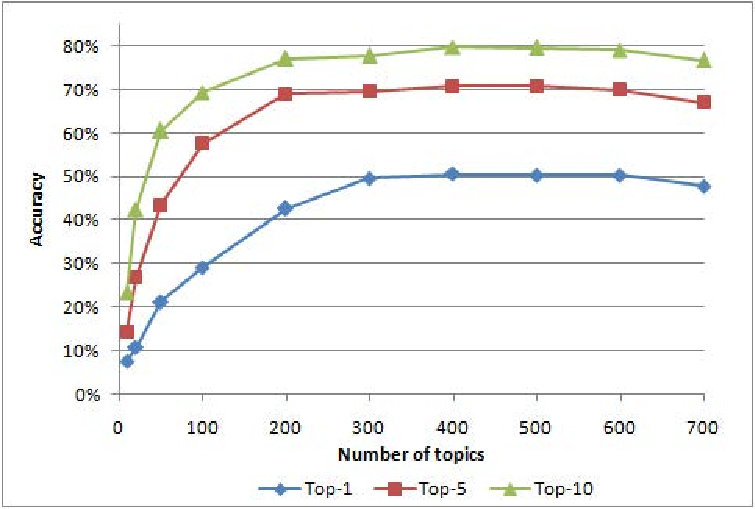
\includegraphics[width=3.3in]{sensitive}
\caption{Top-ranked Accuracy with Different Numbers of Topics for Eclipse}
\label{sensitive}
\end{figure}

%%\begin{figure}
%%\centerline{\epsfxsize=3.3in \epsffile{tradeoff.eps}}
%%\caption{Top-ranked Accuracy with Different Numbers of Sampling Size}
%%\label{tradeoff}
%%\end{figure}

\begin{table}[t]
\centering
\caption{Top-ranked Accuracy with Different Sampling Sizes $r$}
\setlength{\tabcolsep}{2.5pt}
\begin{tabular}{|l||r|r|r|r|r|r|r|r|r|r|r|r|r|}
\hline
   r(\%) & 0 & 1 & 5 & 10 & 20 & 30 & 40 & 50 & 60 & 70 & 80 & 90 & 100\\
\hline
   Top-1 (\%) & 47 & 48 & 48 & 49 & 50 & 51 & 51 & 51 & 51 & 51 & 51 & 52 & 52\\
   Top-5 (\%) & 67 & 67 & 69 & 69 & 70 & 70 & 71 & 71 & 71 & 71 & 72 & 72 & 72\\
   Top-10 (\%) & 75 & 75 & 77 & 79 & 79 & 80 & 80 & 81 & 80 & 81 & 81 & 81 & 81\\
\hline
   Time (s) & 17 & 22 & 38 & 58 & 111 & 146 & 190 & 235 & 280 & 330 & 370 & 406 & 477\\
\hline
\end{tabular}
\label{tradeoff}
\end{table}

In our next experiment, we evaluated the sensitivity of accuracy as
the size $r$ of (Gibbs) sampling set varies for incremental updating
of {\model}'s internal data (Section~\ref{updating-algo}). We fixed
the number of topics $K$ at 500 because we used Eclipse data set for
this experiment. We varied the size of the sample set from 0, 1, 5,
10, 20, ..., 90, and 100\% of the full size of existing data. The case
of 100\% means complete re-training. We measured accuracy and the
updating time for each case. As seen in Table~\ref{tradeoff}, when the
sample size of bug reports used for updating the internal model is
small, time efficiency is gained very much with very little accuracy
reduced. For example, with the selection of 10\% of previous bug
reports for model updating, the updating time is 8.2 times smaller but
top-ranked accuracy reduces only from 2-3\%. This result shows that
our selection strategy for a smaller sample set
(Section~\ref{updating-algo}) for incremental updating is efficient
and quite accurate. If a small sample of previous bug reports is
selected such that all duplicate ones are included, accuracy will not
reduce much.


\subsection{Accuracy Comparison}

\begin{figure}[t]
\centering
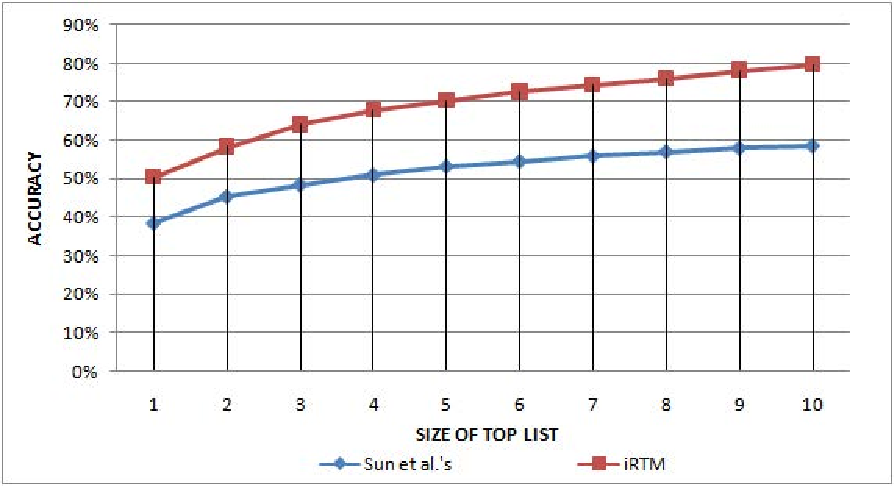
\includegraphics[width=3.3in]{eclipse3}
\caption{Accuracy Comparison with Different Top List Sizes for Eclipse}
\label{eclipse}
\end{figure}


In the next experiment, we compared {\model}'s performance with that
of Sun {\em et al.}'s~\cite{davidlo10}. The parameters of {\model} in
this experiment were selected after fine-tuning for best results as
described earlier. Figure~\ref{eclipse} displays the accuracy result
of {\model} in comparison with Sun {\em et al.}'s on Eclipse data
set. As shown, for a new bug report, {\bf in half of the detection cases,
{\model} can correctly detect the duplication (if any) with just a
single result}. With a list of top 5 resulting bug reports, {\model}
can correctly detect the duplication of a given report in 71\% of the
cases. That is, given a bug report, it can correctly detect its
duplication(s) (if any) within its top-5 recommended bug reports in
almost 3 out of 4 cases. With top lists of 10 reports, it can correctly
detect in 80\% of the cases. In comparison, Sun {\em et al.}'s tool
can achieve the accuracy levels at the top lists of sizes 5 and 10 at
only 53\% and 58\%, respectively. In general, for top lists from 1-10
bug reports, {\bf {\model} achieves higher accuracy than Sun {\em et al.}'s
from 12--22\%}.

\begin{figure}[t]
\centering
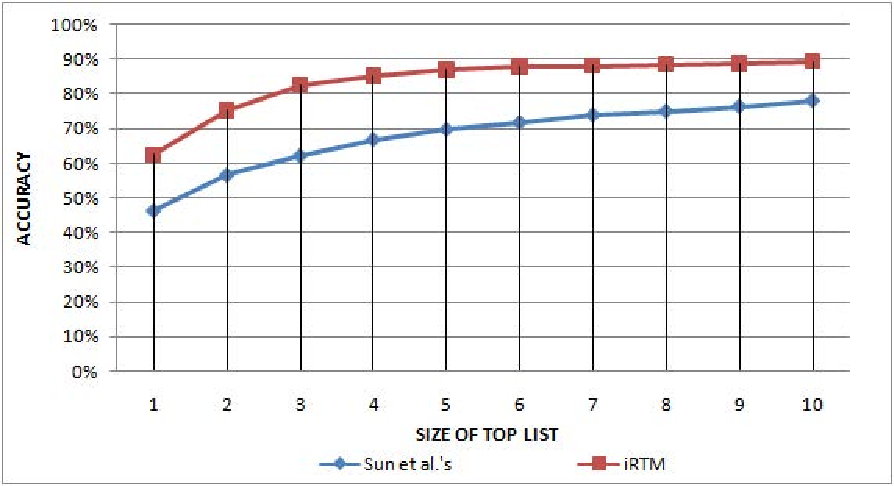
\includegraphics[width=3.3in]{openoffice}
\caption{Accuracy Comparison with Different Top List Sizes for OpenOffice}
\label{openoffice}
\end{figure}

%\begin{figure}[t]
%\centerline{\epsfxsize=3.3in \epsffile{openoffice.eps}}
%\caption{Accuracy Comparison with Different Top List Sizes for OpenOffice}
%\label{openoffice}
%\end{figure}

Figures~\ref{openoffice}, \ref{firefox}, \ref{apache},
\ref{freedesktop}, and \ref{netbeans} display the accuracy results of
    {\model} in comparison with Sun {\em et al.}'s approach on
    OpenOffice, FireFox, Apache, FreeDesktop, and NetBeans datasets,
    respectively. {\bf {\model} consistently achieves very high levels
      of accuracy (with up to 63\% for top-1, 87\% for top-5, and 90\%
      for top-10 accuracy)}. On average for each subject system, the
    top-1, top-5, and top-10 accuracy levels are 56\%, 78\%, and 85\%,
    respectively. For the top-1 to top-10 results, {\bf {\model}
      consistently outperformed Sun {\em et al.}'s with higher
      accuracy from 6--25\%} (from 11--20\% on OpenOffice, 4--9\% on
      FireFox, 6--11\% on Apache, 18--25\% on FreeDesktop, and
      6--11\% on NetBeans datasets).


%%Figure~\ref{openoffice} displays the accuracy result of {\model} in
%%comparison with Sun {\em et al.}'s on OpenOffice data set. As seen,
%%{\model} consistently has very high level of accuracy (63\%, 87\%, and
%%90\% for top-1, top-5, and top-10 accuracy). For the top-1 to top-10
%%results, {\model} achieves higher accuracy than Sun {\em et al.}'s
%%approach from 11\%-20\%.

\begin{figure}[t]
\centering
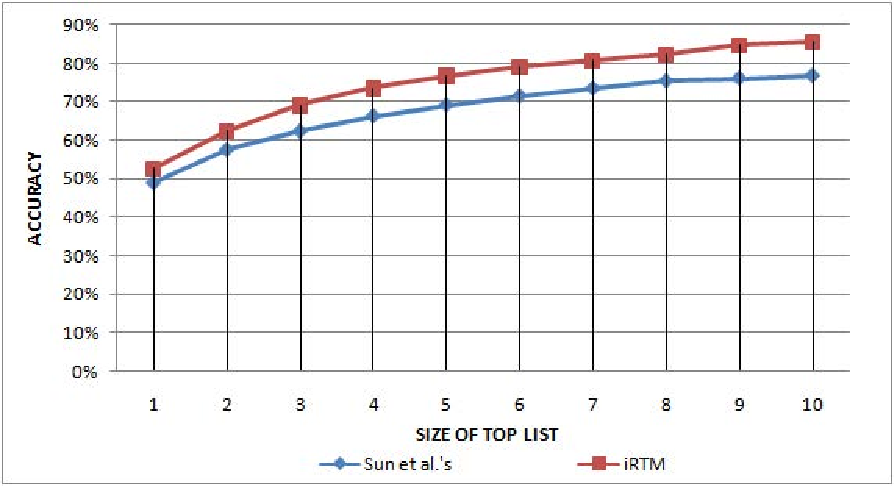
\includegraphics[width=3.3in]{firefox2}
\caption{Accuracy Comparison with Different Top List Sizes for FireFox}
\label{firefox}
\end{figure}

%%Figure~\ref{firefox} displays the accuracy result of {\model} in
%%comparison with Sun {\em et al.}'s on FireFox dataset. As shown,
%%{\model} achieves a higher level of accuracy than their approach. With
%%top lists of 5 and 10 reports, it can correctly determine in 77\% and
%%86\% of the cases, respectively. In comparison, the corresponding
%%numbers at top-5 and top-10 in Sun {\em et al.}'s approach is 70\% and
%%77\%. For the top-1 to top-10 results, {\model} achieves higher
%%accuracy than Sun {\em et al.}'s from 4\%-9\%.

\begin{figure}[t]
\centering
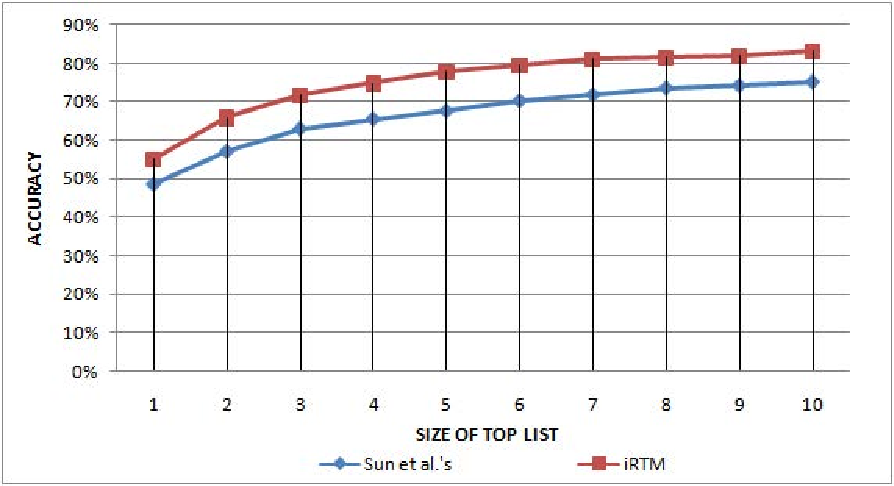
\includegraphics[width=3.3in]{apache}
\caption{Accuracy Comparison with Different Top List Sizes for Apache}
\label{apache}
\end{figure}

%%Figure~\ref{apache} shows {\model}'s accuracy on Apache dataset. As
%%seen, {\model} achieves higher accuracy than Sun {\em et al.}'s
%%from 6\%-11\%. Importantly, it consistently has very high accuracy
%%(78\% and 83\% top-5 and top-10 accuracy).

\begin{figure}[t]
\centering
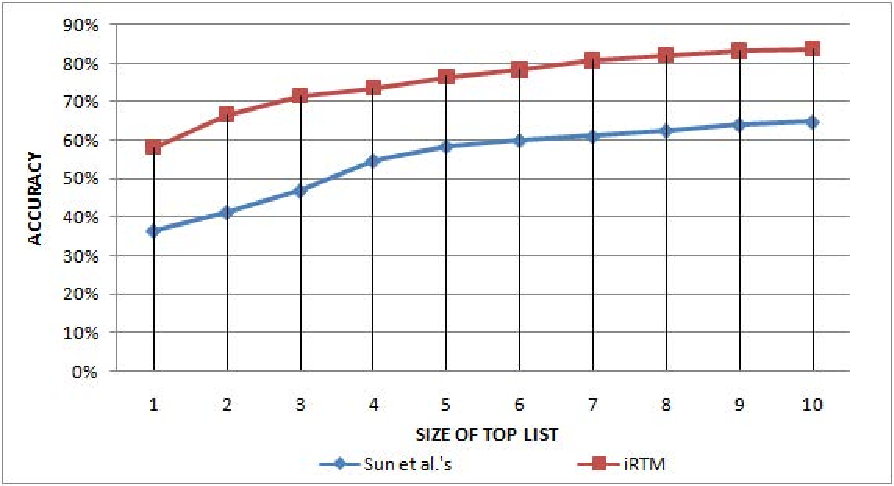
\includegraphics[width=3.3in]{freedesktop}
\caption{Accuracy Comparison with Different Top List Sizes for FreeDesktop}
\label{freedesktop}
\end{figure}

%\begin{figure}[t]
%\centerline{\epsfxsize=3.3in \epsffile{freedesktop.eps}}
%\caption{Accuracy Comparison with Different Top List Sizes for FreeDesktop}
%\label{freedesktop}
%\end{figure}

%%Similarly higher level accuracy was achieved on FreeDesktop dataset
%%for {\model} as shown in Figure~\ref{freedesktop} (77\% top-5 and 84\%
%%top-10 accuracy). For this dataset, {\model} outperformed Sun {\em et
%%al.}'s from 18\%-25\% for top-1 to top-10 lists of results. {\model}
%%also achieves a higher level of accuracy than their approach on the
%%NetBeans dataset (Figure~\ref{netbeans}).

\begin{figure}[t]
\centering
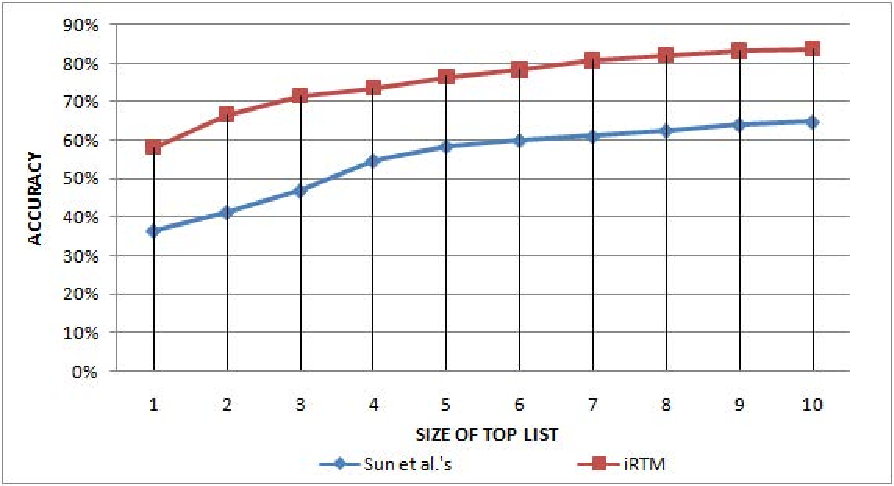
\includegraphics[width=3.3in]{freedesktop}
\caption{Accuracy Comparison with Different Top List Sizes for NetBeans}
\label{netbeans}
\end{figure}

\subsection{Time Efficiency Comparison}

\begin{table*}[t]
\centering
\footnotesize
\caption{Time Efficiency Comparison}
\begin{tabular}{|l||r|r|r|r||r|r|r|r|}
  \hline
     &  & {\model} & & & & Sun's &  & \\
  \hline
  Project & Initial & Average & Update & Prediction & Initial & Average & Re-Training & Prediction \\
          & Training & Update & per Report  & & Training & Re-Training & per Report  & \\
  \hline
  Eclipse & 850s & 150s & 0.25s & 1.7s & 810s & 860s & 1.4s & 25s\\
  OpenOffice & 485s & 65s & 0.09s & 1.4s & 334s & 350s & 0.5s & 18s \\
  FireFox & 1,280s & 182s & 0.09s & 4.3s & 1,350s & 1,420s & 0.7s & 73s\\
  Apache  & 711s & 88.5s & 0.08s & 1.7s & 491s & 522s & 0.53s & 36s \\
  FreeDesktop & 833s & 93.5s & 0.09s & 2.1s & 546s & 576s & 0.58s & 43s\\
  NetBeans & 953s & 181.5s & 0.18s & 2.7s & 972s & 1,024s & 1s & 67s\\
  \hline
\end{tabular}
\label{timetab}
\end{table*}

%\begin{table}[t]
%\centering
%\footnotesize
%\caption{Time Efficiency Comparison}
%\begin{tabular}{|l||r|r|r||r|r|r|}
%  \hline
%     &  & {\model} & & & Sun's &  \\
%  \hline
%  Project & Initial & Update & Pred. & Initial & Re-Train & Pred. \\
%          & Train &  &  & Train &  & \\
%  \hline
%  Eclipse & 850s & 150s & 17s & 810s & 860s & 25s\\
%  FireFox & 1,280s & 182s  & 43s & 1,350s & 1,420s & 73s\\
%  OpenOffice & 485s & 65s & 13.5s & 334s & 350s & 18s \\
%  \hline
%\end{tabular}
%\label{timetab}
%\end{table}

During running two tools on the collected data sets, we also recorded
the execution time. Table~\ref{timetab} displays the result. Column
\code{Initial Training} shows the amount of initial training time of
the corresponding tool for the first data frame. Column \code{Average
Update} displays the average updating time for {\model} for each data
frame. In contrast, Sun {\em et al.}'s needs to re-train the data and
its average re-training time for each frame is in the column
\code{Average Re-Training}. Column \code{Update per Report} shows the
updating time for each bug report for {\model}, while column
\code{Re-training per Report} is for average re-training time per bug
report in Sun {\em et al.}'s. Column \code{Prediction}
shows the corresponding prediction time for each bug report.

{\model} is much more efficient than Sun {\em et al.}'s SVM approach,
especially for large datasets. {\model} took much shorter time (many
times faster) for data updating than complete re-training time in
their approach. On average, for a new bug report, it took only about
0.14s for {\model} to update its data.
%The training time in {\model} is proportional to the number of bug
%reports as we will show it later.
The complete re-training time in Sun {\em et al.}'s is in fact higher
than that of its initial training because in later data frames, more bug
reports were included. That is, the more bug reports come, the higher
its complete re-training time will be.

%For the model updating with 120 new bug reports, it took only 1 hour
%in training for {\model}. For a new bug report, it took only 30
%seconds for duplication detection.

\subsection{Scalability}

In our third experiment, we evaluated the scalability of {\model}
for a large data set. In this experiment, we prepared a larger dataset
of Eclipse's bug reports with a longer history. We chose Eclipse's
platform component  with 61,110 bug
reports, in which 14,020 are determined by Eclipse's developers as
duplicate ones.  The sizes of vocabulary sets is 120,372 terms. 
%(In the previous experiment for comparing {\model} with Sun {\em et
%  al.}'s approach, we did not use this data set because SVM cannot
%scale.)

Figure~\ref{time} shows the dependence between training time and the
number of bug reports in Eclipse's dataset. As shown, the amount of
training time increases almost linearly with respect to the number of
bug reports and their duplicate indicators (We keep the number of
iterations of Gibbs sampling the same). This is a key advantage of
{\model} over the SVM-based model in Sun {\em et al.}~\cite{davidlo10}
where the complete training time increases significantly as the number
of bug reports increases. Importantly, the update time with
incremental training is much smaller than that of the complete
re-training, and {\model} still scales well as the number of bug
reports increases.

\begin{figure}[t]
\centering
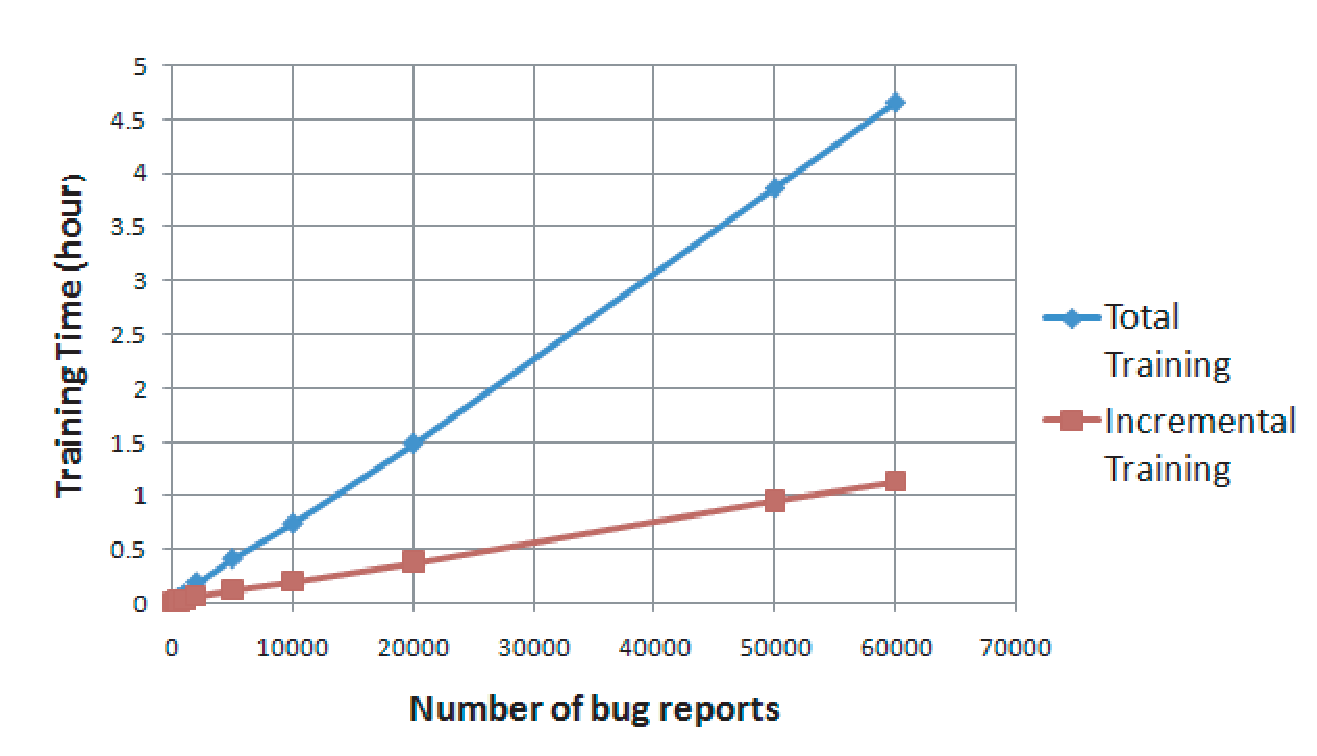
\includegraphics[width=3.5in]{time}
\caption{Training Time for Eclipse's Data}
\label{time}
\end{figure}

%begin{figure}[t]
%centerline{\epsfxsize=3.5in \epsffile{time.eps}}
%caption{Training Time for Eclipse's Data}
%label{time}
%end{figure}

%Importantly, to compare the result from an incremental run with that
%of a fully re-training run, we compared the detection results after 7,
%14, 21, and so on frames between two runs. In all cases, both runs
%gave no significantly different results.

%\subsection{Threats to Validity}

 %\subsection{Interesting Case Studies}

%Let us discuss a few real-world examples that we found during our
%experimental studies.



%Figure {\ref{bugreport225337}} shows two duplicate bug reports
%detected by {\model}. Except the terms NPE
%(\code{NullPointerException}) and \code{StructuredViewer}, which are
%popular and common in the project, the two reports contain several
%different terms because the reporters found the bug in two different
%usage scenarios. That leads to different exception traces: one
%involving image updating, and another on widget selection. We noticed
%that when running BM25F model by itself, bug report \#225169 is ranked
%8$^{th}$ in the list that could be duplicate of bug report \#225337
%due to the dissimilarity in texts. However, after extracting topics
%via the co-occurrences of other terms such as \code{startup},
%\code{first time}, \code{RSE perspective}, \code{wizard}, etc in the
%previous duplicate reports (e.g. from bug report \#218304, not shown),
%{\model} ranked it at the highest position and detected them as
%duplicate ones.

%\begin{figure}
%\vspace{2mm}
%\sf
%\small
%
%\textbf{Bug Report \#225169}\\
%\textbf{Summary}:  Get NPE when startup RSE on a new workspace\\
%\textbf{Description}:\\
%	Using Eclipse M5 driver and RSE I20080401-0935 build. Start
%	eclipse on a new workspace, and switch to RSE perspective. I
%	could see the following error in the log. But
%	otherwise, things are normal.\\ java.lang.NullPointerException
%	at\\
%	org.eclipse.....getImageDescriptor(SystemView...java:123)\\
%	...\\ at
%	org.eclipse....doUpdateItem(AbstractTreeViewer.java:1010)\\ at
%	org.eclipse....doUpdateItem(SafeTreeViewer.java:79)\\ at
%	org.eclipse....run(StructuredViewer.java:466)...\\
%	-----------------------------------------------------------------------\\
%\textbf{Bug Report \#225337}\\
%\textbf{Summary}:  NPE when selecting linux connection in wizard for the first time\\
%\textbf{Description}:\\
%	After starting an eclipse for the first time, when I went select Linux in the
%	new connection wizard, I hit this exception.  When I tried again a few times
%	later, I wasn't able to hit it.\\
%	java.lang.NullPointerException at\\
%	org.eclipse....getAdditionalWizardPages(RSEDefault...:404)\\
%	...\\
%	at org.eclipse....updateSelection(StructuredViewer.java:2062)\\
%	at org.eclipse....handleSelect(StructuredViewer.java:1138)\\
%	at org.eclipse....widgetSelected(StructuredViewer.java:1168)...\\
%\caption{Duplicate Bug Reports in Eclipse}
%\label{bugreport225337}
%\end{figure}

%-------------------------------------------------------------------------
% SECOND EXAMPLE
%-------------------------------------------------------------------------

\begin{figure}[t]
%\scriptsize
%\sf
\small
\textbf{Bug Report \#240790}\\
\textbf{Summary}: [search] callers are not found when caller and callee reside in sibling Java projects\\
\textbf{Description}:\\
	1. create a java project "common" having one interface\\...
	6. Client.init() is not found being a caller (search cope might be
	"Workspace" or "Hierarchy")\\
-----------------------------------------------------------------------\\
\textbf{Bug Report \#250454}\\
\textbf{Summary}:   [search] Cannot find method references between projects\\
\textbf{Description}:\\
	1) define 3 projects: rootProject, subProject1, and subProject2.\\
	2) set project build depedencies such that subProject1 and subProject2 depend
	on rootProject...\\
	6) Search for references to Square.f() directly from it's declaration in
	Square.java.\\
			6a) EXPECT: one result: ShapeUser.useShape(Shape)\\
			6b) ACTUAL: no results\\
	If ShapeUser is instead located in the direct derivable project dependency
	graph for subProject1, the results are ok....\\
			1) If Square were defined in rootProject itself, the search succeeds.\\
			2) If Square were defined in subProject2, the search succeeds. \\
			3) If subProject2 has a build dependency on subProject1, the search
	succeeds.\\

	Additionally, searching for references to f() from the Shape declaration
	succeeds as defined above.  It appears the search does not go to all dependent
	projects of the project declaring the interface....\\
\caption{Duplicate Bug Reports \#250454 and \#240790}
\label{bugreport250454}
\end{figure}

\vspace{0.04in}
\noindent {\bf Interesting Case Studies} An example of detected duplicate bug reports 
is in Figure~\ref{bugreport250454}. The texts in two summaries are
different. The re-producing steps described by two bug reporters are
totally different. As running with the Sun {\em et al.}'s model alone, bug
report \#240790 was ranked 6th in the list of potential duplications
of bug report \#250454. Trained with historical data via identified
duplicate reports of \#250454 (not shown), DBTM can learn sets of
different terms describing the same technical issue in this new
report, which is the issue of searching objects dependent on sibling
projects.

%Final
%More examples are shown on our project's web site.
%(\url{http://home.engineering.iastate.edu/~anhnt/Research/DBTM/})

%, real duplicate group (bug report \#240790) of bug report \#250454 is
%ranked sixth in the ranked list of BM25f model because the two bugs do
%not has much text similarity (they only share important word
%\code{search}).  The duplicate group is ranked first in our experiment
%using DBTM, since the model can learn that the two bug reports
%\#240790 and \#250454) infer to the issue when searching objects on
%dependent (sibling) projects.

%We also find hundreds of cases where DBTM can elevate the ranked of
%real duplicate group in the ranked list of potential duplicate groups
%of a bug report, in comparison with BM25f model. See our website for
%our finding.


\vspace{0.04in}
\noindent {\bf Threats to Validity.}  We evaluated only on six
open-source projects in which three of them are from an existing work
on duplication bug report detection. We cannot ensure {\model} will
work well in other projects where different projects might have
different quality of bug reports.  However, Eclipse, Mozilla and
OpenOffice are long-lasting projects and were used in prior
research. They are sufficiently representative for our comparison. We
also should validate our method on commercial projects.

%
%For comparison, we re-implemented the SVM technique in Sun {\em et
%  al.}~\cite{davidlo10}, rather using their tool (which is not
%available). However, we followed exactly their description in their
%paper~\cite{davidlo10}, and used the same machine learning tool
%LIBSVM~\cite{libsvm} as in their work to re-implement it.


%The training time is a function of number of bug reports, number of
%duplicate links, number of iterations of Gibbs sampling.
%However, through experiment, the value is almost a linear function of
%the number of bug reports and the number of duplicate links.
%When the number of of duplicate links increases, iRTM ensures that the
%training time not increasing explosively.
%The update time when we use the incremental mechanism is even more
%faster. Figure (~\ref{time}) shows the dependence of update time as a
%function of number of samples used for random Gibbs sampling and the
%size of bug reports.



%\begin{figure}[h]
%	\includegraphics[width=3.6in,angle=270]{TrainingTime1.eps}
%	\caption{Training time for Eclipse}
%	\label{fig:TrainingTime1}
%\end{figure}

%Comparing with Sun {\em et al.}'s approach~\cite{davidlo10}, their
%average accuracy levels at the top lists of sizes 5,10, and 20 are
%41\%, 60\%

